\begin{myTheorem}[Diagonal dominance theorem]  
Given a unit disk partitioned into $n\ge2$ shells and limbs, and two integer $k$ such that $1\le k < j \le n$.
%%%
\begin{equation}
  A_{kk} > A_{jj}
\end{equation}
%%%
\label{eq:limb dom}
\end{myTheorem}  %  -  -  -  -  -  -  -  -  -  -  -  -  -  -  -  -
\begin{proof}  %  +  +  +  +  +  +  +  +  +  +  +  +  +  +  +  +
Employ a Matryoshka doll strategy by nesting the areas as shown in figure \eqref{fig:Matryoshka}.
\begin{figure}[htbp] %  figure placement: here, top, bottom, or page
   \centering
   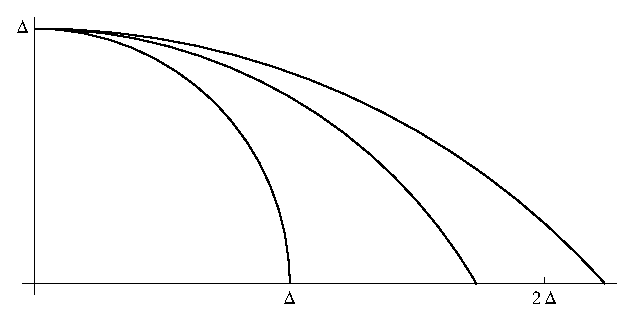
\includegraphics[ width = 3in ]{graphics/Matryoshka.eps} 
   \caption{Nesting the areas of interest. This is the family of curves in \eqref{eq:Matryoshka} for $k=1,2,3$.}
   \label{fig:Matryoshka}
\end{figure}
The equation for curve $y_{k}(x)$ is
  % = =  e q u a t i o n
  \begin{equation}
    y_{k}(x) = \sqrt{(k \Delta)^{2} - x^{2}} - (k-1)\Delta, \quad 0\le x \le \sqrt{2k-1} .
    \label{eq:Matryoshka}
  \end{equation}
  % = =
Over this domain the curve $y\ge0$. For the proof it is sufficient to show dominance over the shared domain. Given integers $j$ and $k$ such that $1\le j < k \le n$ one must prove that
  % = =  e q u a t i o n
  \begin{equation}
    y_{k}(x) \ge y_{j}(x), \qquad 0\le x \le \sqrt{2k-1} .
    \label{eq:yk gt yj}
  \end{equation}
  % = =
Subtracting the Maclauren expansions leads to
  % = =  e q u a t i o n
  \begin{equation}
    y_{k}(x) - y_{j}(x) 
      = \sum_{m=1}^{\infty} \binom{1/2}{m} \frac{x^{2m}}{\Delta^{2m-1}}\paren{\frac{1}{j^{2m-1}}-\frac{1}{k^{2m-1}}} .
   \end{equation}
  % = =
By postulation, $j>k$ and each of these terms is shell positive which establishes \eqref{eq:yk gt yj}.
\end{proof}  %  +  +  +  +  +  +  +  +  +  +  +  +  +  +  +  +

\endinput %-------------------------------